\documentclass{article}

\usepackage[margin=1.35in]{geometry}
\usepackage{algorithm2e}
\usepackage{amsfonts}
\usepackage{amsmath}
\usepackage{forest}
\usepackage{hyperref}
\usepackage{mathtools}
\usepackage{tikz}

\usetikzlibrary{arrows}
\usetikzlibrary{positioning}

\title{R1CS Programming \\ \large ZK0x04 Workshop Notes}
\author{Daniel Lubarov \and Brendan Farmer}
\date{\today}

\DeclarePairedDelimiter\ceil{\lceil}{\rceil}
\DeclarePairedDelimiter\floor{\lfloor}{\rfloor}

% Hyperlink colors.
\hypersetup{
    colorlinks=true,
    linkcolor=blue,
    citecolor=blue,
    urlcolor=blue,
}

% Tweak autoref names to use capitals.
\renewcommand{\sectionautorefname}{Section}
\renewcommand{\subsectionautorefname}{Section}
\renewcommand{\subsubsectionautorefname}{Section}

\begin{document}

\maketitle

{\hypersetup{hidelinks} \tableofcontents}
\newpage


\section{Multiplicative inverse} \label{sec:inverse}

Deterministically computing $1 / x$ in an R1CS circuit would be expensive. Instead, we can have the prover compute $1 / x$ outside of the circuit and supply the result as a witness element, which we will call $x_\mathrm{inv}$. To verify the result, we enforce
\begin{equation}
  (x) (x_\mathrm{inv}) = (1)
\end{equation}


\section{Zero testing} \label{sec:zerotest}

To assert $x = 0$, we simply enforce
\begin{equation}
  (x) (1) = (0)
\end{equation}
Asserting $x \ne 0$ is similarly easy: we compute $1 / x$ (non-deterministically, as in \autoref{sec:inverse}). The result can be ignored; the mere fact that an inverse exists implies $x \ne 0$.

On the other hand, if we want to \textit{evaluate}
\begin{equation} \label{eq:nonzero}
  y \coloneqq
  \begin{cases}
    0 & \text{if $x = 0$,} \\
    1 & \text{otherwise,}
  \end{cases}
\end{equation}
we can do so by introducing another variable, $m$, and enforcing
\begin{alignat}{2}
  (x)     & (m) &&= (y), \\
  (1 - y) & (x) &&= (0).
\end{alignat}
Outside of the circuit, the prover generates $y$ as in \autoref{eq:nonzero}, and generates $m$ as
\begin{equation}
  m \coloneqq
  \begin{cases}
    1 & \text{if $x = 0$,} \\
    y / x & \text{otherwise.}
  \end{cases}
\end{equation}
This method is from \cite{parno2013pinocchio}.

We can also use this technique to test for equality, since $x = y$ if and only if $x - y = 0$.


\section{Binary}

To assert $b \in \{ 0, 1 \}$, we enforce
\begin{equation} \label{eq:boolean}
  (b) (b - 1) = (0).
\end{equation}

To ``split'' a field element $x$ into its binary encoding, $(b_1, \dots, b_n)$, we have the prover generate the binary encoding out-of-band. We then verify it by applying \autoref{eq:boolean} to each $b_i$, and enforcing
\begin{equation} \label{eq:binary}
  (x) (1) = \left( \sum_{i=0}^{n-1} 2^i b_i \right),
\end{equation}
assuming a little-ending ordering of the bits.

Note that \autoref{eq:binary} permits two encodings of certain field elements. In $\mathbb{F}_{13}$ for example, the element $1$ can be represented as either $0001$ or $1110$. If a canonical encoding is required, we can prevent ``overflowing'' encodings by asserting that $(b_1, \dots, b_n) < |F|$. Such binary comparisons are covered in \autoref{sec:comparisons}.

To ``join'' a sequence of bits into the field element they encode, we simply take a weighted sum of the bits:
\begin{equation} \label{eq:join}
  x \coloneqq \sum_{i=0}^{n-1} 2^i b_i.
\end{equation}
This does not require any constraints, unless we don't know whether $(b_1, \dots, b_n)$ is the canonical encoding of some field element, in which case we may want a comparison to assert that overflow does not occur.


\section{Selection} \label{sec:selection}

Suppose we have a boolean value $s$, and we wish to compute
\begin{equation}
  z \coloneqq
  \begin{cases}
    x & \text{if $s = 0$,} \\
    y & \text{if $s = 1$.}
  \end{cases}
\end{equation}
We can compute this as
\begin{equation} \label{eq:selection}
  z \coloneqq x + s(y - x).
\end{equation}
This requires two constraints: one ``is boolean'' assertion (\autoref{eq:boolean}), assuming $s$ was not already known to be boolean, and another for the multiplication.


\section{Random access} \label{sec:random-access}

Suppose we wish to access the $i$th item of some sequence $(x_0, \dots, x_n)$. There are several variations of this problem, but for the sake of brevity, we will assume that
\begin{enumerate}
  \item The sequence length is a power of two: $n = 2^k$.
  \item The items are individual field elements (rather than, say, elliptic curve points).
  \item Each item $x_j$ is a constant.
\end{enumerate}
We start by splitting $i$ into its binary encoding, $(i_0, \dots, i_k)$. One may think of $(i_0, \dots, i_k)$ as a path through a binary tree, where $i_j$ indicates the direction of descent at height $j$. For example, say $n=8$ (thus $k=3$) and $i = 5 = 101$. This corresponds to the following binary tree:
\begin{center}
\begin{forest}
  for tree={circle,draw,inner sep=0,minimum size=0.6cm},
  selected/.style={edge={red,thick},draw={red,thick}}
  [,selected
    [,
      [,
        [$x_0$],
        [$x_1$]
      ],
      [,
        [$x_2$],
        [$x_3$]
      ]
    ],
    [,selected,
      [,selected,
        [$x_4$],
        [$x_5$,selected]
      ],
      [,
        [$x_6$],
        [$x_7$]
      ]
    ]
  ]
\end{forest}
\end{center}
Now, we will describe a few methods of random access which build upon this mental model.


\subsection{Repeated selection method}

First, we could perform a selection operation (\autoref{sec:selection}) for each non-leaf node. In the example, we would perform the following operations:
\begin{center}
\begin{forest}
  for tree={draw,inner sep=2mm,minimum size=0.6cm},
  [{$r = \operatorname{sel}(b_2, z_0, z_1)$},
    [{$z_0 = \operatorname{sel}(b_1, y_0, y_1)$},
      [{$y_0 = \operatorname{sel}(b_0, x_0, x_1)$},
        [$x_0$],
        [$x_1$]
      ],
      [{$y_1 = \operatorname{sel}(b_0, x_2, x_3)$},
        [$x_2$],
        [$x_3$]
      ]
    ],
    [{$z_1 = \operatorname{sel}(b_1, y_2, y_3)$},
      [{$y_2 = \operatorname{sel}(b_0, x_4, x_5)$},
        [$x_4$],
        [$x_5$]
      ],
      [{$y_3 = \operatorname{sel}(b_0, x_6, x_7)$},
        [$x_6$],
        [$x_7$]
      ]
    ]
  ]
\end{forest}
\end{center}
after which the root node $r$ will hold $x_i$. This involves $n - 1$ (or $2^k - 1$) selection operations, since a perfect tree with $n$ leaves contains $n - 1$ non-leaf nodes. However, if $(x_0, \dots, x_n)$ are constant then selecting between two leaves becomes a free linear combination, which brings the cost down to $n/2 - 1$ (or $2^{k - 1} - 1$) constraints.


\subsection{Sum-of-conditions method}

Alternatively, we could construct an expression for each node which encodes the conditions under which that node, or one of its ancestors, is selected. In the example, we have
\begin{center}
\begin{forest}
  for tree={draw,inner sep=2mm,minimum size=0.6cm},
  [{$1$},
    [{$1 - b_2$},
      [{$(1 - b_2) (1 - b_1)$},
        [{\ldots}],
        [{\ldots}]
      ],
      [{$(1 - b_2) b_1$},
        [{\ldots}],
        [{\ldots}]
      ]
    ],
    [{$b_2$},
      [{$b_2 (1 - b_1)$},
        [{\ldots}],
        [{\ldots}]
      ],
      [{$b_2 b_1$},
        [{\ldots}],
        [{\ldots}]
      ]
    ]
  ]
\end{forest}
\end{center}
Then to access $x_i$, we take the sum of each leaf multiplied by its selection condition. Note that this final multiplication is free, given our assumption that $(x_0, \dots, x_n)$ are constants.

Computing these conditions naively would require $n - 1$ constraints, since we would perform one multiplication per non-root node. We can achieve much greater efficiency, however, by distributing the products and reusing intermediate products. In the example, we would compute just four products: $b_0 b_1$, $b_0 b_2$, $b_1 b_2$, and $b_0 (b_1 b_2)$. In general, the cost of this approach is $2^k - k - 1$ constraints.


\subsection{Hybrid method} \label{sec:random-access-hybrid}

Unfortunately, both of the aforementioned methods cost $\mathcal{O}(n)$ constraints. It turns out that we can do better by combining them. Pick some $l, m$ such that $l + m = k$. We divide our conceptual tree into subtrees of size $2^l$, and apply the sum-of-conditions method to each subtree. This costs $2^l - l - 1$ constraints independent of the number of subtrees, since each subtree uses the exact same set of conditions.

Next, we invoke the selection method to select one of the $2^m$ subtree results. This costs another $2^m - 1$ constraints, for a total cost of $2^m + 2^l - l - 2$. By picking $l = m = k/2$, we obtain a total cost of $\mathcal{O}(\sqrt{n})$ constraints.


\section{Embedded curve operations}

Embedded curves have several uses in SNARKs. A few examples are Schnorr signatures, Pedersen hashes, and recursive SNARK verifiers.
Here we will focus on twisted Edwards curves such as Jubjub.


\subsection{Addition}

Recall the addition law for twisted Edwards curves,
\begin{equation}
  (x_1, y_1) + (x_2, y_2) = \left( \frac{x_1 y_1 + y_1 x_2}{1 + d x_1 x_2 y_1 y_2}, \frac{y_1 y_2 - a x_1 x_2}{1 - d x_1 x_2 y_1 y_2} \right).
\end{equation}
Applying the law directly takes 7 constraints: 4 for the products in the numerators, one for the product in the denominator, and one\footnote{In general, computing a quotient $q \coloneqq x / y$ takes two constraints: $(y) (y_\mathrm{inv}) = (1)$ and $(x) (y_\mathrm{inv}) = (q)$. In this case, however, we can multiply both sides by the denominator since we know it will never be zero. This yields a single constraint: $(q) (y) = (x)$.} for each of the two quotients. This can be optimized to 6 constraints as described in \cite{hopwood2016zcash}.

However, the operation becomes much cheaper when of the points is constant. Without loss of generality, suppose $(x_1, y_1)$ is constant while $(x_2, y_2)$ is variable. Then the numerators become ``free'' linear combinations, while the denominators require a single multiplication. The quotients add 2 constraints as before, resulting in 3 constraints total.

Finally, when doubling a point, the addition law simplifies to
\begin{equation}
  [2] (x, y) = \left( \frac{2 x y}{a x^2 + y^2}, \frac{y^2 - a x^2}{2 - a x^2 - y^2} \right)
\end{equation}
which requires 5 constraints.


\subsection{Multiplication}

Consider the problem of computing $[s] p$, where $p$ is a constant point and $s$ is a variable scalar. A simple, reasonably efficient approach is known as multiplication by doubling. We split $s$ into its binary encoding, $(s_0, \dots, s_n)$, then compute
\begin{equation} \label{eq:mult-by-doubling}
  [s] p = \sum_{i=0}^{n-1} [s_i] [2^i] p.
\end{equation}
Since $p$ is constant, $[2^i] p$ can be precomputed. Thus for each $i$, we perform a conditional addition: if $s_i = 1$, we add $[2^i] p$ to an accumulator. Since adding a constant point is cheaper than adding a variable point, it is best to structure the computation as
\begin{center}
\begin{algorithm}[H]
  \SetKwData{Sum}{sum}
  \SetKwFunction{Select}{select}
  $\Sum \leftarrow 0$\;
  \For{$i \leftarrow 0$ \KwTo $n$}{
    $q \leftarrow \Sum + [2^i] p$\tcc*{addition with a constant value}
    $\Sum \leftarrow \Select(s_i, \Sum, q)$\;
  }
  \Return \Sum\;
\end{algorithm}
\end{center}
Ignoring the cost of splitting, this requires 5 constraints per bit: 3 for the constant addition, and 2 for selecting a 2-tuple.


\subsubsection{Windowed multiplication}

We can generalize \autoref{eq:mult-by-doubling} by decomposing $s$ into its base-$2^w$ encoding, rather than base 2 specifically. Let $(s_0, \dots, s_{n/w})$ be the base-$2^w$ decomposition of $s$. Note that $s_i$ can be expressed as a linear combination of bits of $s$, so the cost of decomposition does not change. We can rewrite $[s] p$ as
\begin{equation}
  [s] p = \sum_{i=0}^{n/w-1} [s_i] [(2^w)^i] p.
\end{equation}
As before, $[(2^w)^i] p$ can be precomputed for each $i$. We can go a step further by precomputing $[s_i] [(2^w)^i] p$ for each of $2^w$ possible values of $s_i$, then looking up the relevant value using the method described in \autoref{sec:random-access-hybrid}.

In practice, a window size of 3 seems optimal. If we configure our random access gadget with $l = 2$ and $m = 1$, the lookup costs 3 constraints per 3-bit window.\footnote{This is one more than the formula in \autoref{sec:random-access-hybrid} would imply, since the selection operation needs to be done for both coordinates of the curve point.} The addition adds another 6 constraints per window, for a total cost of 9 constraints per window, or $3$ constraints per bit.


\section{2x2 switch}

Suppose we wish to implement a switch with the following structure:
\begin{center}
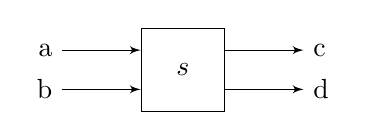
\begin{tikzpicture}[node distance=1.0cm,auto,>=latex']
  \node [draw, minimum size=3em] (s) {$s$};
  \node (a) [left=of s.155] {a};
  \node (b) [left=of s.205] {b};
  \node (c) [right=of s.25] {c};
  \node (d) [right=of s.335] {d};
  \draw[->] (a) -- (s.155);
  \draw[->] (b) -- (s.205);
  \draw[->] (s.25) -- (c);
  \draw[->] (s.335) -- (d);
\end{tikzpicture}
\end{center}
In particular, if $s = 0$ then the outputs should be identical the inputs: $(c, d) = (a, b)$. If $s = 1$ then the inputs should be swapped: $(c, d) = (b, a)$.

This requires two constraints: one ``is boolean'' assertion (\autoref{eq:boolean}), and another for selecting the value of $c$ (\autoref{eq:selection}). Once we have $c$, we can compute $d$ as
\begin{equation}
  d \coloneqq a + b - c
\end{equation}
which does not require any additional constraints.


\section{Permutations} \label{sec:permutations}

Say we want to verify that two sequences, $(x_1, \dots, x_n)$ and $(y_1, \dots, y_n)$, are permutations of one another. This can be done efficiently using routing networks, which used a fixed (for a fixed $n$) network of 2x2 switches.

AS-Waksman networks \cite{beauquier2002arbitrary} are a particularly useful construction, since they support arbitrary permutation sizes. They use about $n \log_2(n) - n$ switches, which is close to the theoretical lower bound of $\log_2(n!)$.


\section{Sorting}

Like permutation networks, sorting networks use a fixed network of gates. In particular, a sorting network is comprised of several 2x2 comparator gates, each of which takes two inputs and sorts them. It is theoretically possible to construct a sorting network for $n$ elements using $\mathcal{O}(n \log n)$ gates \cite{ajtai19830}, but practical constructions use $\mathcal{O}(n \log^2 n)$ gates. Since each comparison adds $\mathcal{O}(\log |F|)$ constraints, this approach is fairly expensive.

A better solution is to leverage non-determinism: instead of creating an R1CS circuit to sort a sequence, we have the prover supply the ordered sequence. Using a permutation network (\autoref{sec:permutations}), we can efficiently verify that the two sequences are permutations of one another. Then for each contiguous pair of elements in the ordered sequence, $x_i$ and $x_{i + 1}$, we assert $x_i \le x_{i + 1}$.


\section{Comparisons} \label{sec:comparisons}

Suppose we want to evaluate $x < y$. For now, assume that both values fit in $n$ bits, where $2^{n + 1} < |F|$. We compute
\begin{equation} \label{eq:bounded-comparison}
  z = 2^n + x - y.
\end{equation}
Notice that $2^n$ has a single 1 bit with index $n$, which will be cleared if and only if $x < y$. Thus we split $z$ into $n + 1$ bits, and the negation of the $n$th bit is our result.

If $x$ and $y$ are unbounded, then the aforementioned technique does not apply. A neat solution was described by Ahmed Kosba. First, we split $x$ and $y$ into their binary forms, $(x_0, \dots, x_n)$ and $(y_0, \dots, y_n)$. Next we divide each binary sequence into $c$-bit chunks, and join each chunk of bits into a field element (\autoref{eq:join}).

The prover non-deterministically identifies the most significant chunk index at which $x$ and $y$ differ, if any. We add constraints to verify that the identified chunks do indeed differ, and that any more significant chunks are equal. Finally, we compare the two identified chunks using \autoref{eq:bounded-comparison}.

If we choose $c, l \in \mathcal{O}(\sqrt{n})$, this approach requires $\mathcal{O}(\sqrt{n})$ constraints in addition to the cost of splitting the inputs (if they were not already in binary form). A couple optimizations are possible in particular circumstances:
\begin{enumerate}
  \item To assert (not evaluate) $x < y$, we can split $x$ non-canonically and split $y$ canonically. The prover is forced to use $x$'s canonical encoding anyway, otherwise $x_\mathrm{bin} \ge |F| > y_\mathrm{bin}$, making the assertion unsatisfiable.
  \item To assert $x < c$ for some constant $c \ll |F|$, we can split $x$ into just $\ceil{\log_2 c}$ bits.
\end{enumerate}


\bibliography{bibliography}{}
\bibliographystyle{ieeetr}

\end{document}
